%% Suggestion dom:
%% Plus fluide
%% Résultats plus punché et vendre
%% Timestep par années
%% Diapo conclu
%% Ajouter +4

\documentclass[10pt,aspectratio=149]{beamer}

\usecolortheme{Calm}
\usetheme{Calm}

%%\usepackage{minted}
%%\usemintedstyle{pastie}

\usepackage{pgfplots}
\usepackage{pgfplotstable}
\usepackage[utf8]{inputenc}
\usepackage{mathpazo}
\usepackage{xcolor}

\usetikzlibrary{shapes, arrows, positioning}

\setbeamertemplate{itemize items}[circle]

\setbeamerfont{alerted text}{series=\bfseries}
\setbeamertemplate{caption}{\insertcaption} \setbeamertemplate{caption label separator}{}

\author{Steve Vissault, Matthew Talluto, \\
Isabelle Boulangeat and Dominique Gravel}
\title{Does Temperate forest will migrate faster \\ enough to track climate change ?}
\date{\today}
\institute{Université du Québec à Rimouski}


\begin{document}
\begin{frame}[plain]
   \titlepage
\end{frame}


%%%%%%%%%%%%%%%%%%%%%%%%%%%%%%%%%%%%%%%%%%%%%%%%%%%%%%%%%%%%%%%%%%%%%%%%%%%%%%%%%%%%%%%%%%%%%%

\begin{frame}{Context}{The boreal-temperate ecotone}

The surface of the boreal-temperate forests ecotone is \textbf{expected to shift over the next 100 years}.

\begin{figure}
	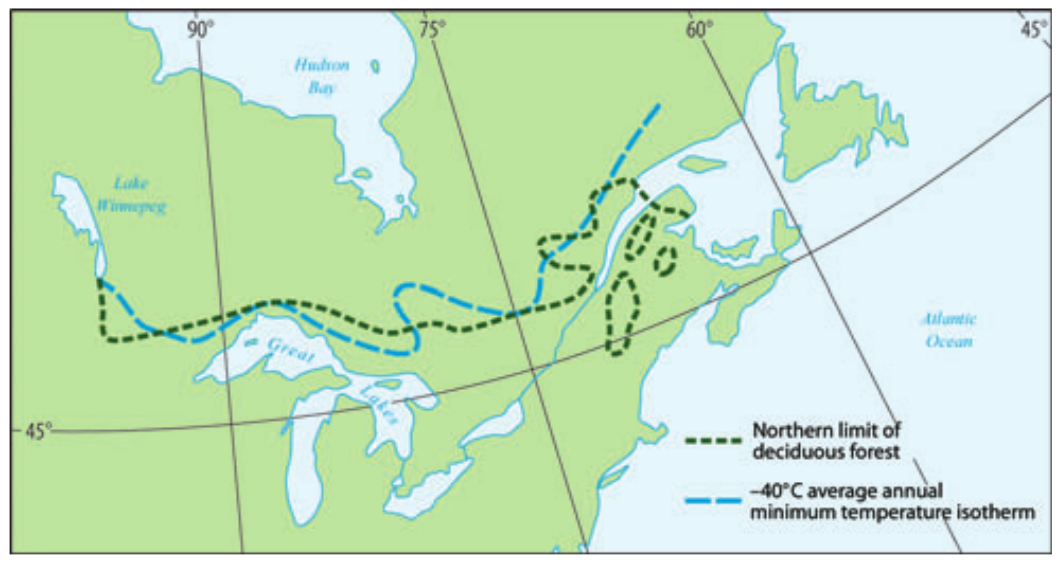
\includegraphics[width=.70\paperwidth]{Figs/climecotone.png}
\end{figure}

   \paper{Goldblum and Rig, 2010}
\end{frame}

%%%%%%%%%%%%%%%%%%%%%%%%%%%%%%%%%%%%%%%%%%%%%%%%%%%%%%%%%%%%%%%%%%%%%%%%%%%%%%%%%%%%%%%%%%%%%%

\begin{frame}{Model approach}{States and Transitions Model}

\begin{columns}[t]
	\begin{column}[t]{.40\paperwidth}
		\begin{figure}
			\small{\input{Figs/fig_wo_params.tikz}}
		\end{figure}
	\end{column}
	\begin{column}{.50\paperwidth}
	\textbf{Model Description}
		\begin{itemize}
			\item Lanscape scale
			\item \textbf{4 States:}
			\begin{itemize}
				\item \textcolor{Temperate}{\textbf{T}}, Temperate
				\item \textcolor{Boreal}{\textbf{B}}, Boreal
				\item \textcolor{Mixed}{\textbf{M}}, Mixed
				\item \textcolor{Regeneration}{\textbf{R}}, corresponds to a post-disturbance
			\end{itemize}
			\item Spatially explicit and stochastic model
		\end{itemize}
	\end{column}
\end{columns}

\end{frame}

%%%%%%%%%%%%%%%%%%%%%%%%%%%%%%%%%%%%%%%%%%%%%%%  %%%%%%%%%%%%%%%%%%%%%%%%%%%%%%%%%%%%%%%%%%%%%%%

\begin{frame}{Results}{Future state distribution predicted}

  \begin{figure}
  	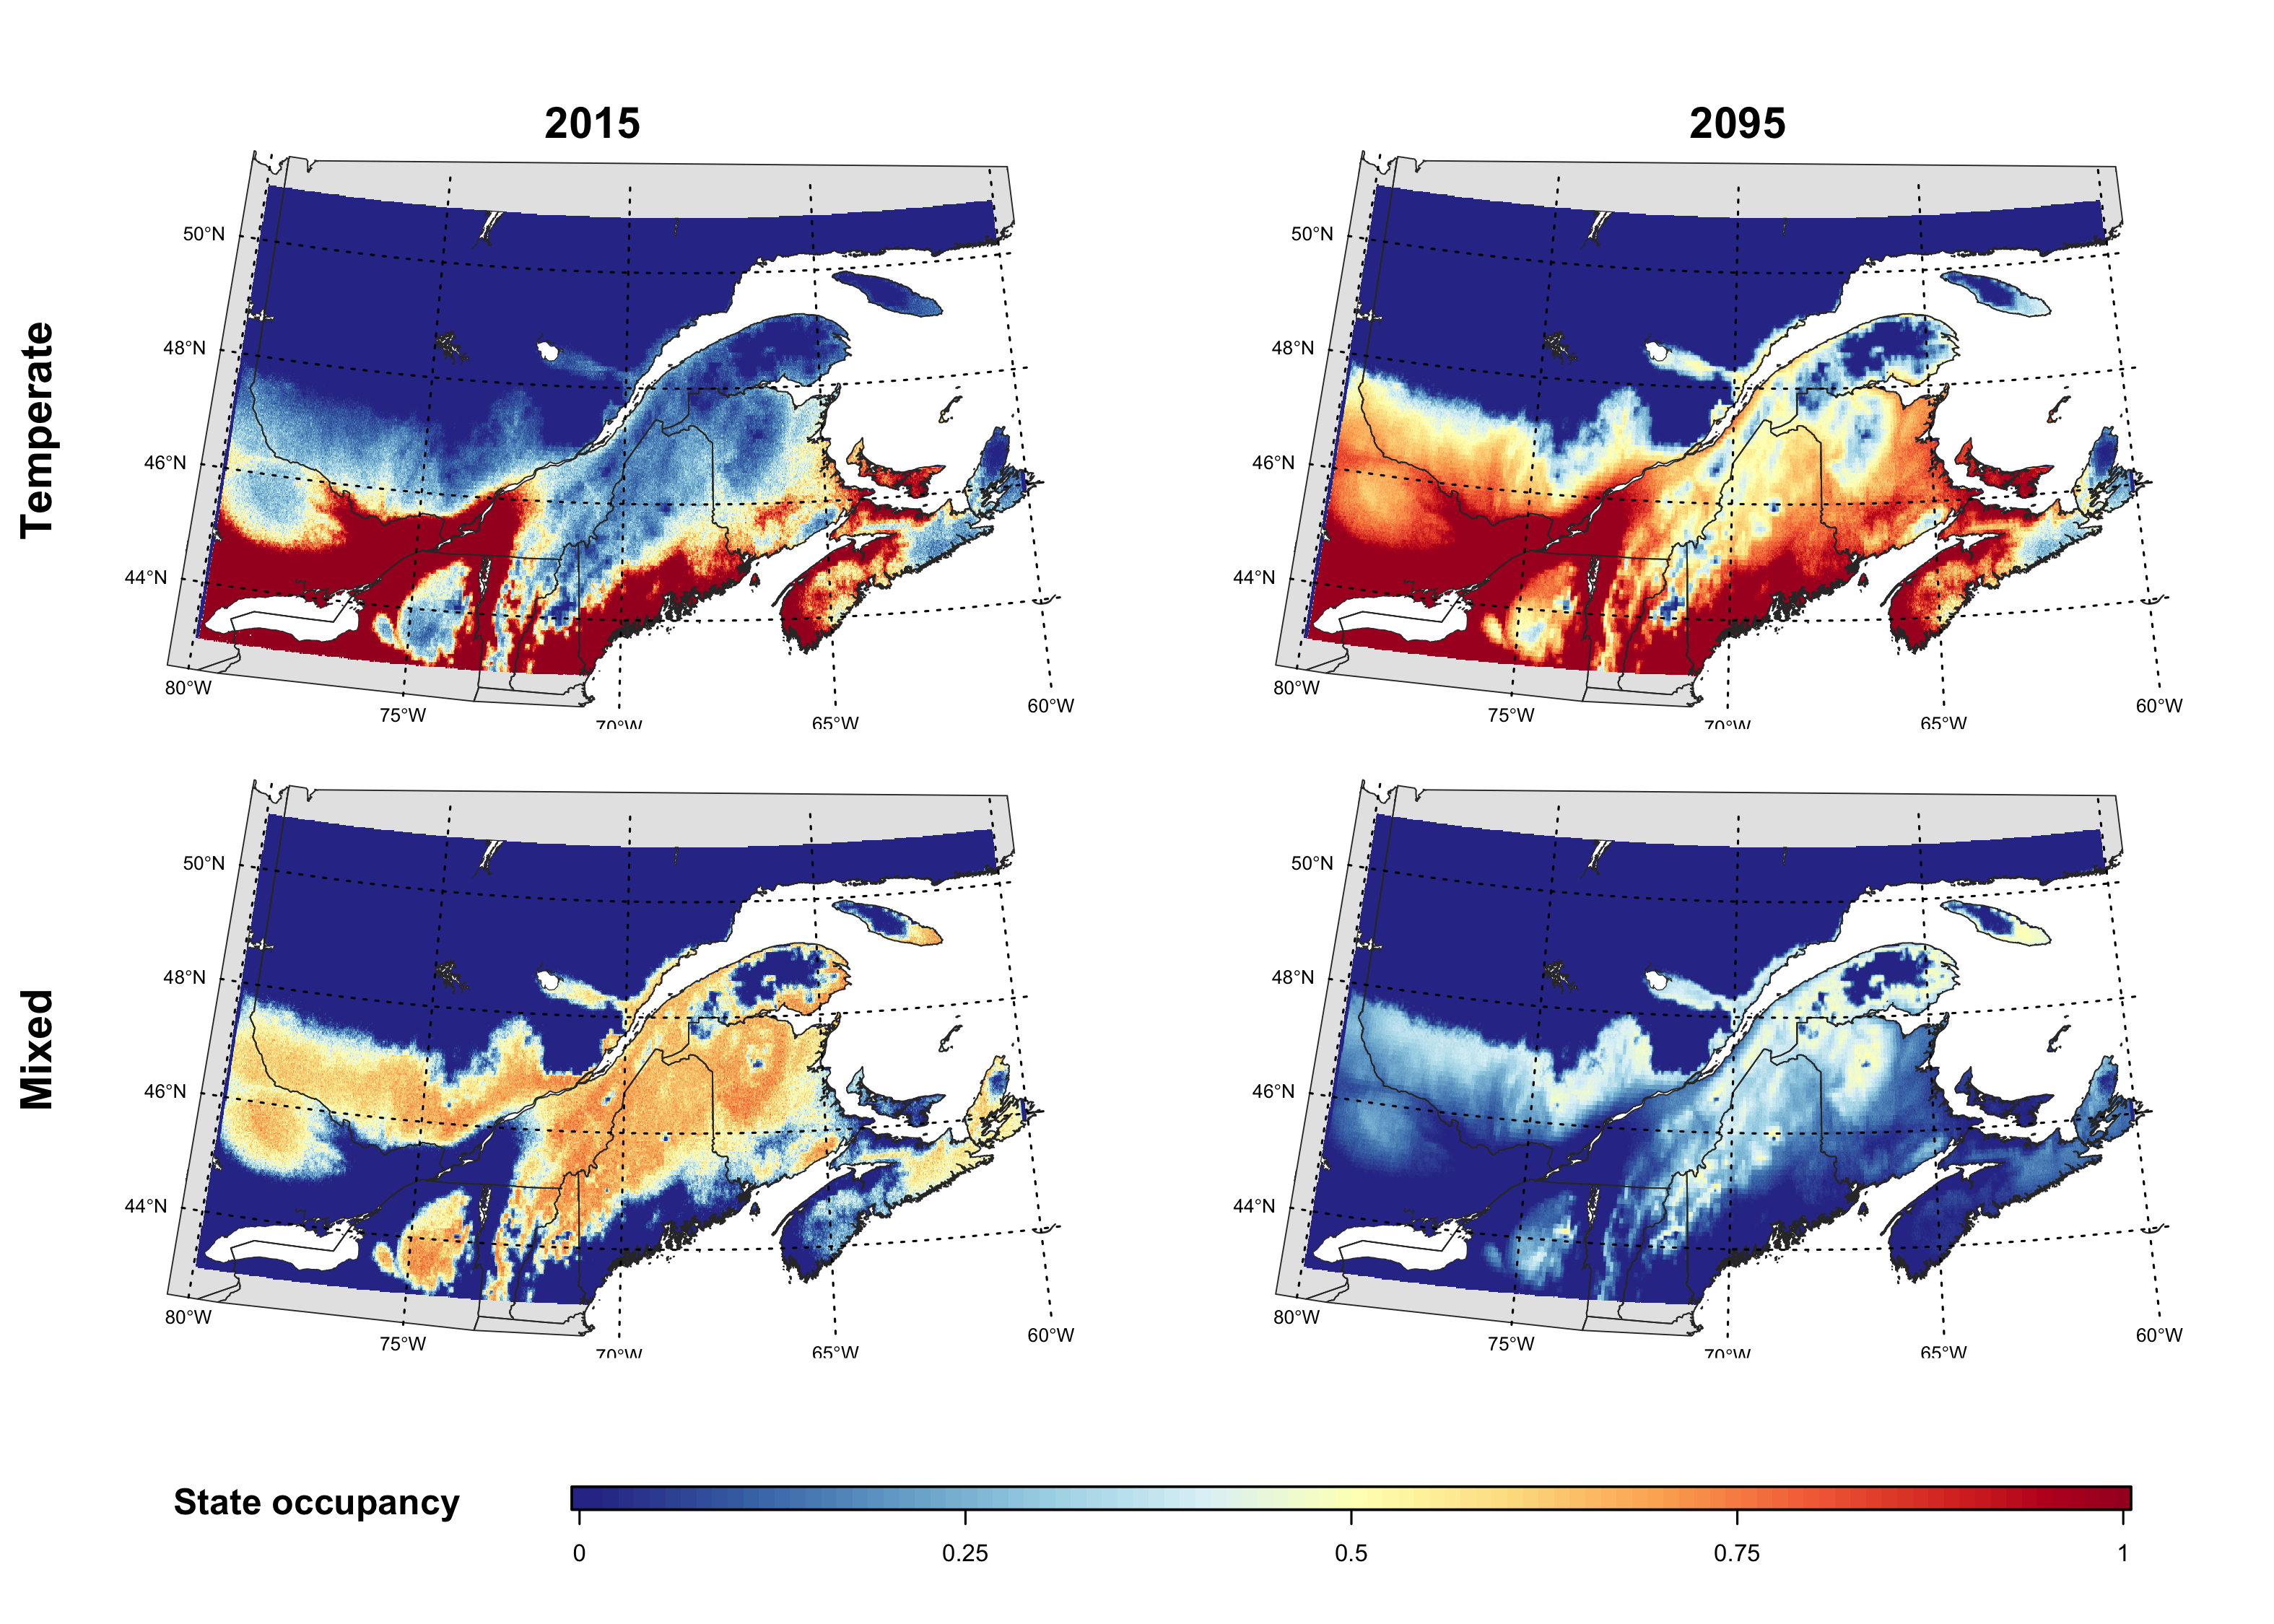
\includegraphics[width=.75\paperwidth]{Figs/future_distrib_states.png}
  \end{figure}

\end{frame}

%%%%%%%%%%%%%%%%%%%%%%%%%%%%%%%%%%%%%%%%%%%%%%%%%%%%%%%%%%%%%%%%%%%%%%%%%%%%%%%%%%%%%%%%%%%%%%

\begin{frame}{Results}{Demography matter}

  \begin{figure}
  	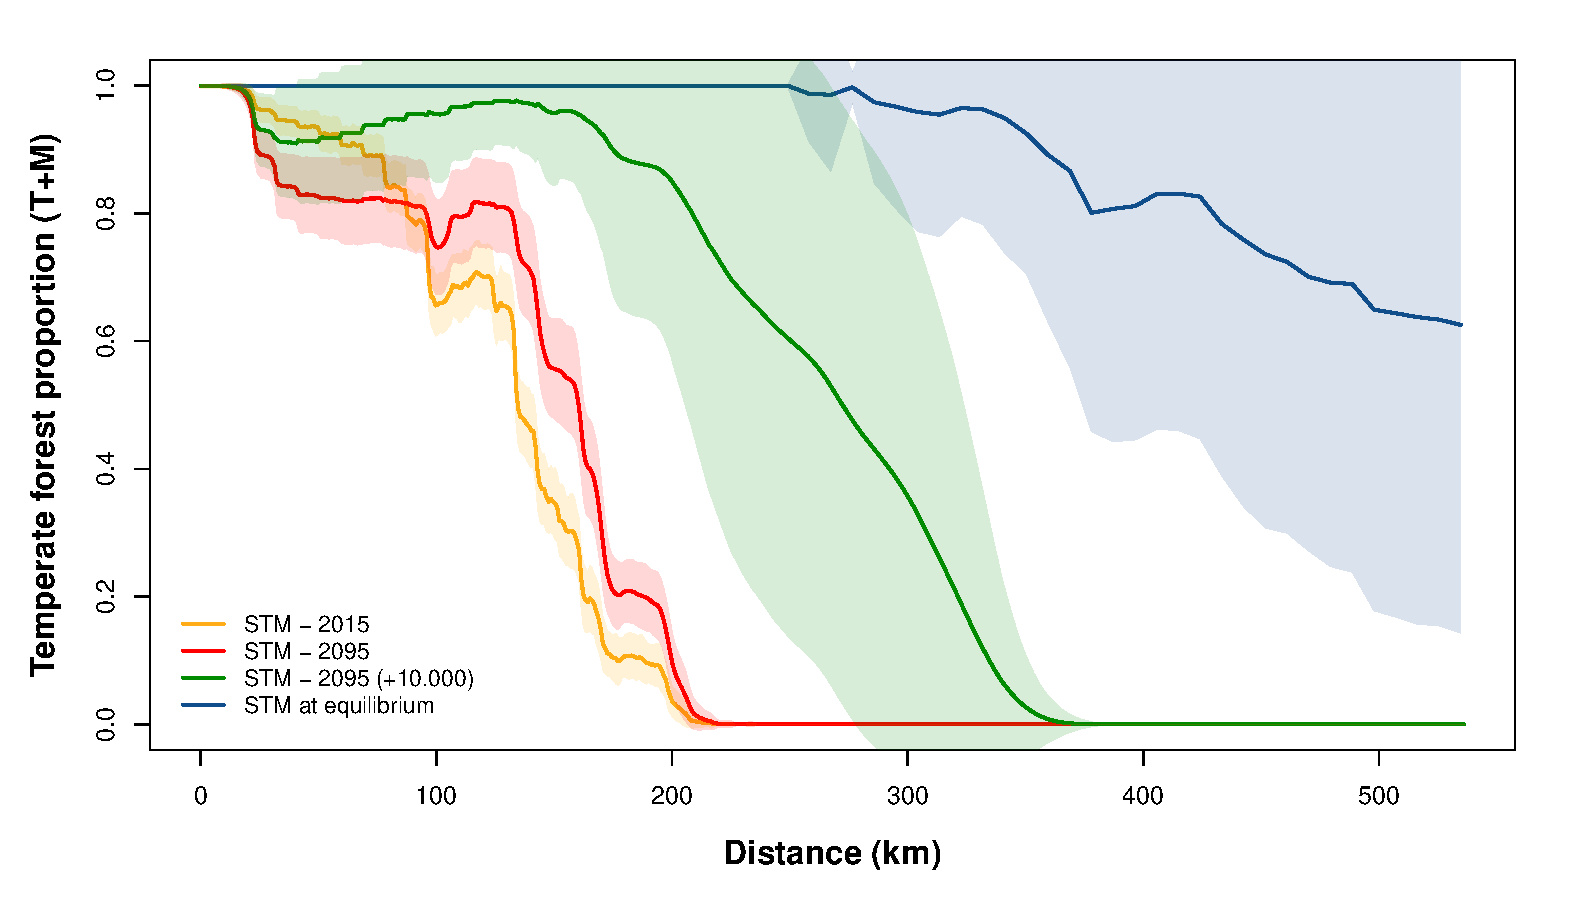
\includegraphics[width=.70\paperwidth]{Figs/propLat_wth_solved.pdf}
  \end{figure}

\end{frame}

%%%%%%%%%%%%%%%%%%%%%%%%%%%%%%%%%%%%%%%%%%%%%%%%%%%%%%%%%%%%%%%%%%%%%%%%%%%%%%%%%%%%%%%%%%%%%%

\begin{frame}[t]{Aknowledgements}
\vspace{-1em}
\begin{center}
		\begin{figure}
			
\includegraphics[width=0.3\paperwidth]{logo.png}
		\end{figure}
		\vfill
		\centering \small{\textbf{Funded by}}
		\vfill
		\begin{figure}
			
\includegraphics[width=0.2\paperwidth]{nserc.png}
		\end{figure}
		\vfill
		\centering \small{\textbf{In collaboration with}}
		\vfill
\begin{columns}[t]
	\begin{column}{0.19\linewidth}
		
\includegraphics[width=0.15\paperwidth]{Figs/logo/logo_11_ORMN.png}
	\end{column}
	\begin{column}{0.19\linewidth}
		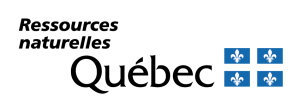
\includegraphics[width=0.15\paperwidth]{Figs/logo/logo_12_MRN.png}
	\end{column}
	\begin{column}{0.22\linewidth}
		
\includegraphics[width=0.21\paperwidth]{Figs/logo/logo_14_CAN.png}
	\end{column}
	\begin{column}{0.17\linewidth}
		
\includegraphics[width=0.12\paperwidth]{Figs/logo/logo_7_domtar.png}
	\end{column}
	\begin{column}{0.17\linewidth}
		
\includegraphics[width=0.13\paperwidth]{Figs/logo/logo_9_ouranos.png}
	\end{column}
\end{columns}
\end{center}
\end{frame}

%%%%%%%%%%%%%%%%%%%%%%%%%%%%%%%%%%%%%%%%%%%%%%%%%%%%%%%%%%%%%%%%%%%%%%%%%%%%%%%%%%%%%%%%%%%%%%

\end{document}
